\chapter{Data sharing and reproducibility: an M/EEG perspective}
\label{chapter:group_study}

\epigraph{\small\itshape ``The first principle is that you must not fool yourself – and you are the easiest person to fool.''}{\small\textit{---Richard Feynman}}

\vspace{20pt}
\epigraph{\small\itshape ``Extraordinary claims require extraordinary evidence.''}
{\small\textit{---Carl Sagan}}

\section{Brain Imaging Data Structure (BIDS)}

While data sharing in neuroscience is on the rise, the amount of data reuse is still limited. For instance, since the release of the Human Connectome Project (HCP)~\citep{larson2013adding} MEG data in 2013, there have been only one or two documented cases~\citep{jas2017autoreject} of reusing the data. Even in these cases, the effort has mostly been to reproduce rather than test new hypotheses. This clearly represents a gap between the ideal of data sharing and the consequences in practice. 

% Clearly, sharing data is not a panacea as the tools, skills and resources to process such large datasets is currently missing in typical laboratories. Perhaps the most important roadblock is standardization of metadata.

\subsection{The need for standards}

\begin{figure}[htb]
\begin{center}
   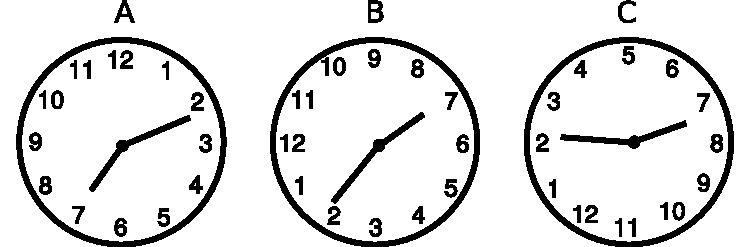
\includegraphics[width=0.7\linewidth]{figures/clock.pdf}
\end{center}
   \caption[Standards in clocks]{Standards in clock design. The time is 07:11 (A) Modern standard, read clockwise and 12 o' clock is at North (B) Anticlockwise and 9 o' clock at North (C) Read clockwise but 5 o' clock is at North. Adapted from \cite{norman2013design}.}
   \label{fig:clock_standards}
\end{figure}
% Data sharing is clearly not productive if the data is not easily  \emph{reusable} in the same way that uncommented and spaghetti code cannot be reused even if it is shared publicly. 
Neuroimaging experiments are often complicated involving different paradigms (auditory, visual, somatosensory \emph{etc.}), different acquisition parameters (sampling frequency, number of sensors and their location, measurement device \emph{etc.}), and population parameters: subject's gender, age \emph{etc.} Obviously, this metadata is necessary information to reanalyze the data.   

Unfortunately, there has been historically, a lack of consensus amongst different labs and industrial manufacturer's as to what constitutes useful metadata. This points to the need for establishing standards. While on a superficial glance, this may appear to be unnecessary bureaucratic red tape, the need for standards can be appreciated by considering the simple wall clocks in Figure~\ref{fig:clock_standards}.

The wall clock is recognized as an everyday object that is perhaps far simpler than most complex neuroimaging experiments. Even then, there are two degrees of freedom even to this simple device: the direction of motion of the hands, and the anchor point for the 12 o' clock. While all three clocks in the figure can still be readable, it is far more convenient to establish a standard. The upfront cost in conforming to the standard is more than made up by the efficiencies achieved as a result of it.

Apart from the metadata that is stored with the data, the data itself is stored amongst one of 10--20 different file formats and at different stages of processing. While there have been some efforts previously to standardize data structures~\citep{gibson2009minimum, grewe2011bottom, stoewer2013singlefile, teeters2015neurodata, bigdely2016preparing}, it has not gained wide acceptability. Designing a new standard is tricky as it requires gaining a community consensus. At the same time it must strike the right balance between rigidity for efficiency and flexibility for adapting to future technologies. 

\subsection{The standard}
The BIDS format is indeed designed with these considerations in mind. The standard involves a hierarchy of folders to describe the imaging technology used, the name of the subject, and the date of the experiment. At each level of hierarchy, files are accompanied by sidecar \code{json} files describing the metadata. These files follow an inheritance principle, that is, a field described in a \code{json} file in a higher level of the hierarchy will be automatically propagated downstream. The main BIDS specification is accompanied by extension specifications which describe specific aspects of describe certain file types. The BIDS consortium is also providing a growing ecosystem of tools to convert datasets into BIDS compatible format as well as to validate data to conform to the standard. 

The development of these standards is going to enable building large databases of neural recordings. In the future, we can envision being able to open a website and query or search through such data by different experimental paradigms or other metadata.

\noindent\fcolorbox{white}{lightgray}{%
\begin{minipage}{\dimexpr\textwidth-2\fboxrule-2\fboxsep\relax}
\begin{itemize}[align=left, leftmargin=10pt, labelwidth=5pt, labelindent=10pt, itemsep=5pt, topsep=5pt]
  \item[] Section~\ref{sec:BIDS-MEG} was published in:
  \item \bibentry{galan2017meg}
\end{itemize}
\end{minipage}}%

\subsection{BIDS}
\label{sec:BIDS-MEG}

\begin{figure}[htb]
\begin{center}
   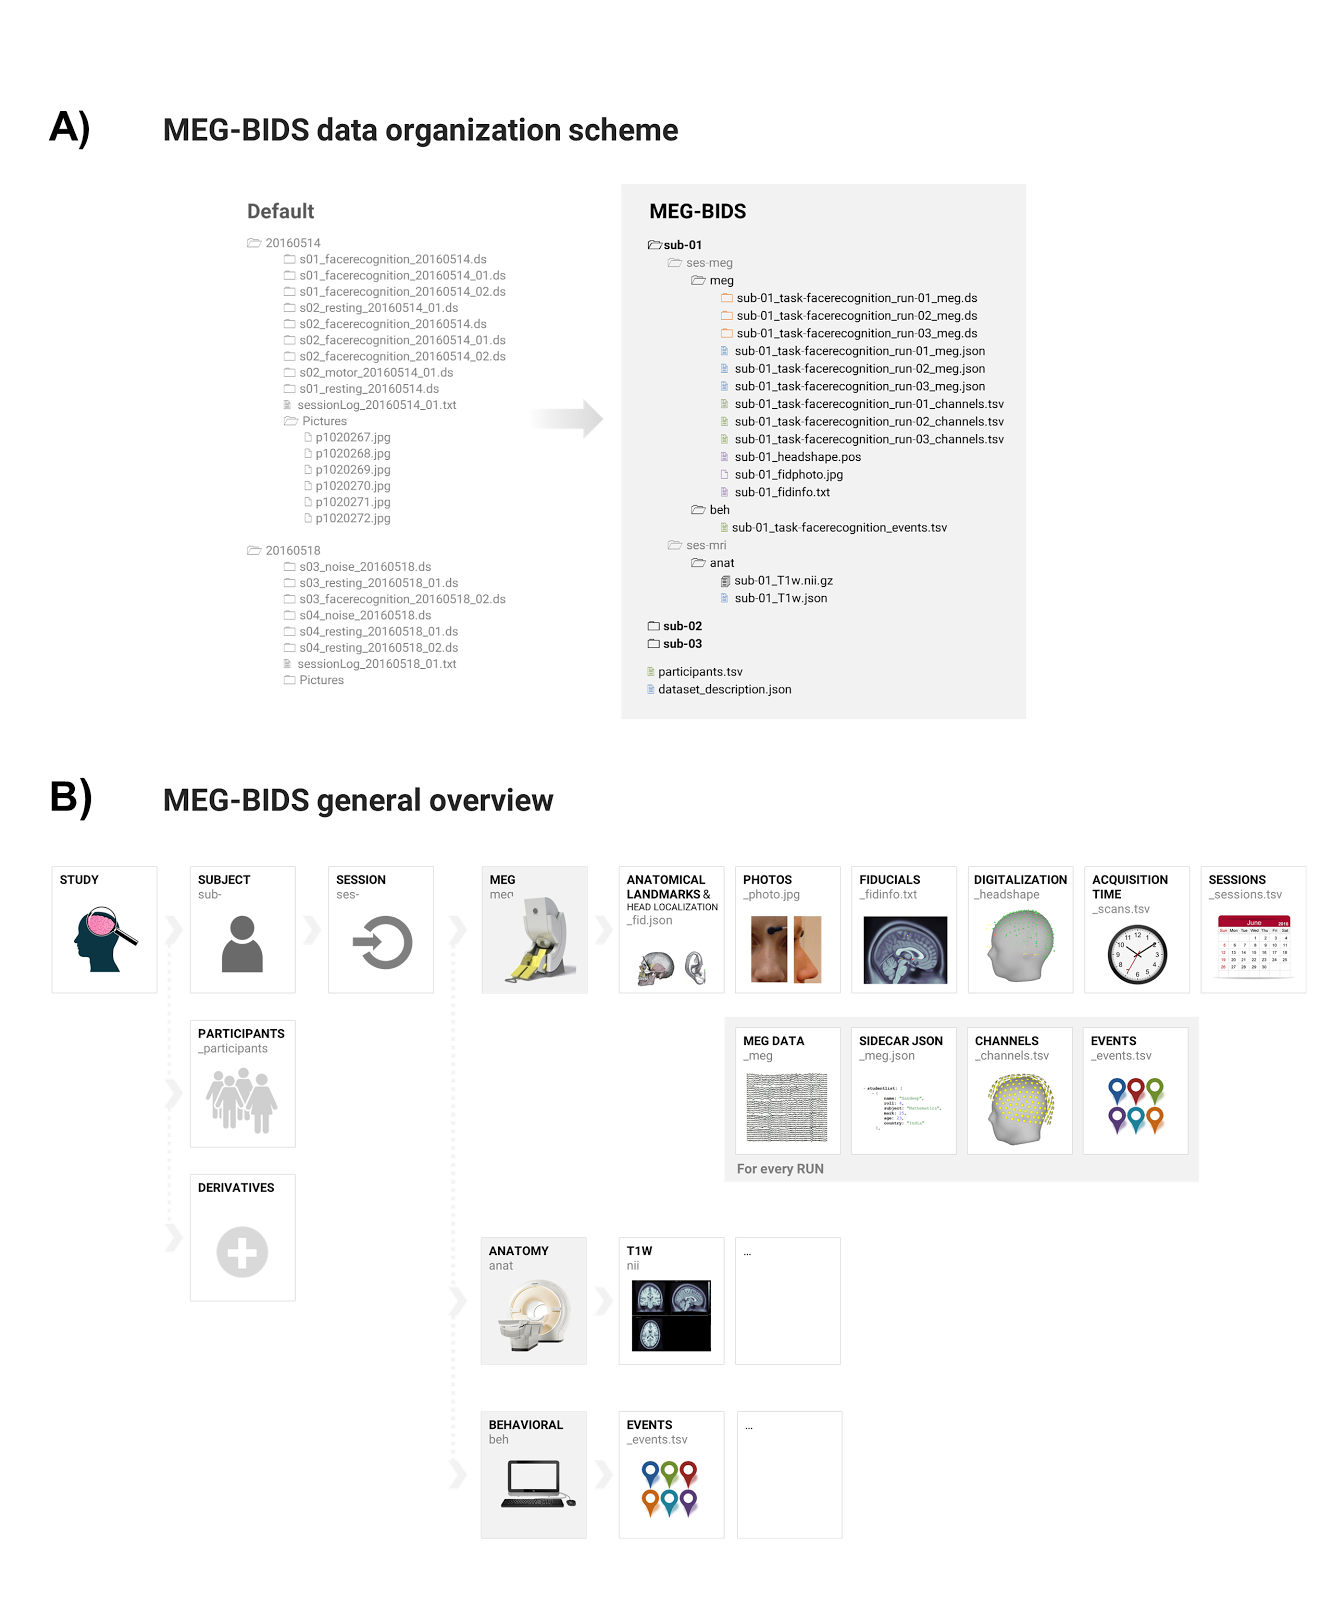
\includegraphics[width=0.5\linewidth]{figures/MEG-BIDS.png}
\end{center}
   \caption[BIDS-MEG data organization scheme.]{ A) BIDS-MEG data organization scheme: Left: a typical default data organization scheme where folder are organized by date of session and contain different runs for a given participant in a study. Right: BIDS-MEG organizes data per study, then participant (subject), followed by modality, then sessions and eventually, runs. Note the sidecar files that are present at all level the data hierarchy, and document conveniently the metadata contents. B) BIDS-MEG general overview}
   \label{fig:BIDS-MEG}
\end{figure}

The BIDS-MEG fields and data organization were defined, bearing in mind best-practice guidelines for conducting MEG research~\citep{gross2013good}. The initiative fostered contributions from multiple MEG experts, with a face-to-face discussion at the 2016 International Conference on Biomagnetism, where the first incarnation of BIDS-MEG was introduced~\citep{niso2016megbids}. The first set of feedback comments and the minutes from further group discussions are publicly available
(\url{https://groups.google.com/d/msg/bids-discussion/xTHBsGhu0hk/MN25xbxRBwAJ}).

A first version of the present manuscript was shared via the preprint server bioRxiv, from where more comments stemming from the community were collected and considered for improvement of BIDS-MEG. A poll survey to probe the interest of the concerned community was also conducted (see main results on Figure~\ref{fig:BIDS-MEG}).

BIDS-MEG builds on the BIDS hierarchical data structure. For instance data descriptors such as subject, session, technique, run are BIDS notions that were re-used in BIDS-MEG. Similarly, the simple although extensively used human and machine readable file formats (JavaScript Object Notation [JSON], and Tab Separated Value [TSV] text files) that contributed to the versatility and practicality of documenting metadata elements in BIDS, were expanded with BIDS-MEG. BIDS-MEG employs a straightforward terminology, cautiously defined in line with the general BIDS specifications, although adapted to the unique requirements of MEG.  For further reference, the BIDS-MEG specifications are detailed in an open-access online document:
\url{https://docs.google.com/document/d/1FWex_kSPWVh_f4rKgd5rxJmxlboAPtQlmBc1gyZlRZM)}

The terms used refer to notions that were defined by reaching a consensus amongst the BIDS-MEG contributors and the MEG community. For example, ‘Subject’ refers to the scanned participant. Note that from a technical standpoint, MEG is not a scanning technique. Yet, we used this terminology for convenience, affinity with other neuroimaging modalities, and to reflect the language used in most MEG labs. A ‘Session’ defines a non-intermittent period of time during which the subject is in the scanner.  A ‘Run’ is a period of time during which empty-room (for noise characterization) or brain activity is recorded continuously, with no interruptions. It is typical with MEG that a session consists of multiple runs: task instructions can change and/or participants can take a break between runs. The notion of ‘Task’ refers to the instructions (and corresponding stimulus material) that are performed by the participant. ‘Responses’ is a feature to indicate the recorded behaviour of the subject in relation to the task.

As with the general BIDS specifications~\citep{gorgolewski2016brain}, BIDS-MEG file names are constituted by a series of key-value pairs, with multiple possible file types. Some  typological aspects are mandatory, while others remain optional, although required to abide to the BIDS guidelines. BIDS-MEG can therefore register data of any kind, including but not limited to task-based, resting-state, and empty-room MEG recordings (e.g., for noise estimation purposes). We emphasize that all of the above notions apply also to EEG, and all modalities of electrophysiology, for which BIDS-MEG serves as template for standardization.  

There is no common, open or standard file format in MEG, equivalent to DICOM or NIfTI in MRI. MEG systems manufacturers (CTF, Elekta/Neuromag, BTi/4D Neuroimaging, KIT/Yokogawa/Ricoh, Tristan Technologies, ITAB, KRISS/Compumedics Neuroscan, York Instruments) all cater a vendor-specific format. With BIDS-MEG, unprocessed (raw) data is stored in the native file format (see Discussion for further consideration of common MEG format initiatives) and users can still rely on their preferred data analysis application, possibly provided by the MEG vendor, to browse and read in the MEG file contents. Software can also extract meta information elements from the raw data files. They concern e.g., data collection parameters and other study descriptors, which are eventually transcribed into sidecar JSON files by said BIDS-MEG compatible applications. One major benefit of metadata extraction is the facilitation of subsequent data searches and indexation, without the handling and repeated parsing of large raw data files. Additional relevant files can be included alongside the MEG raw data: some propositions are detailed in the online specifications.

For a given investigator or research group, BIDS-MEG describes a hierarchical structure that descends from a ‘Study’ folder. Multiple ‘Subject’ subfolders contain the data from the participants enrolled. They are arranged by ‘Session’, each session subfolder containing ‘Run’ folders and eventually, data and metadata files. 

The ‘Run’ folder includes a variety of files: MEG recording files in native format, a sidecar JSON document (\code{*\_meg.json}), a channel description table (\code{*\_channel.tsv}), and other general BIDS files, such as task events tables (\code{*\_events.tsv}) that are likely to be specific of each run. ‘Session’ specific files include the coordinates of anatomical landmarks and head-localization coils stored in a JSON document (\code{*\_fid.json}), optional photographs of the anatomical landmarks and/or head localization coils  (\code{*\_photo.jpg}), fiducials information (\code{*\_fidinfo.txt}), 3-D scalp digitalization files (\code{*\_headshape.<manufacturer\_specific\_format>}) and acquisition times (\code{scans.tsv}). The ‘Subject’ and ‘Study’ specific files are inherited directly from the general BIDS specifications (e.g., participants.tsv). Note that in case of conflict between fields of different runs/sessions, it the inheritance principle should be applied: the description file closer to the data prevails (see Section ‘3.5 The Inheritance Principle’ of the BIDS specifications~\citep{gorgolewski2016brain}.

One issue that required special attention was the multiplicity of coordinate systems and units between MEG systems. To impose a unique coordinate system for BIDS based on the subjects’ brain anatomy (e.g., MNI coordinates or equivalent) was an appealing solution, which however would lack generalizability in the MEG practice. MEG data can be collected without anatomical information, such as empty-room noise recordings, which are important to optimal source modeling~\citep{gross-etal:13}. BIDS-MEG therefore associates all recordings with a coordinate file defined according to the MEG system used. Again, BIDS-MEG compatible software can read and interpret this information properly.

Akin to MRI, we anticipate that the systematic data organization enabled by BIDS-MEG will be supported by an increasing number of neuroimaging tools, and that more shared data repositories will be organized accordingly. The straightforward design of BIDS-MEG makes it an interoperable common exchange format for transferring data between investigators and community repositories e.g., OMEGA~\citep{niso2016omega} and OpenfMRI~\citep{poldrack2017openfmri}. It also facilitates multimodal integration (between MRI, fMRI, MEG, etc), as the data from multiple modalities follow the same organization scheme.

\noindent\fcolorbox{white}{lightgray}{%
\begin{minipage}{\dimexpr\textwidth-2\fboxrule-2\fboxsep\relax}
\begin{itemize}[align=left, leftmargin=10pt, labelwidth=5pt, labelindent=10pt, itemsep=5pt, topsep=5pt]
  \item[] Section~\ref{sec:group_study_intro} to Section~\ref{sec:group_study_discussion} was published in:
  \item \bibentry{jas2017mne}
\end{itemize}
\end{minipage}}%

\section{A reproducible M/EEG group study}
\label{sec:group_study_intro}

% General structure of each section (ideally)
% - Here is what we did
% - Why it makes sense? (figure)
% - This is how we checked that what we did makes sense

\Ac{MEG} and \ac{EEG} are neuroimaging technologies with a high temporal resolution, which provide non-invasive access to population-level neuronal dynamics on virtually any temporal scale currently considered relevant to cognition. % DE that is actually an important point to make. It's a distinct feature of the technology.
While MEG can recover spatial patterns at a higher \ac{SNR} and enjoys a more selective cortical resolution than \ac{EEG}~\citep{baillet17}, EEG is more portable and less expensive, and thus supports the study of cognition in a wider range of situations. Processing M/EEG recordings, however, is inherently challenging due to the multi-dimensional nature of the data, the low \ac{SNR} of brain-related M/EEG signals, and the differences in sensitivity of these measurement techniques. This can give rise to complex sequences of data processing steps which demand a high degree of organization from the investigator.

In an effort to address reproducibility issues recently shown to affect neuroimaging studies~\citep{ioannidis2005most, button2013power,Carp2012,Carp2012289}, a number of community-led efforts have begun developing data sharing~\citep{poldrack2017openfmri} and data organization~\citep{gorgolewski2016brain, galan2017meg} projects. These efforts are necessary first steps, but are not sufficient to solve the problem---they must be complemented by educational tools and guidelines that establish good practices for M/EEG analysis~\citep{gross-etal:13}. However, putting guidelines into practice is not always straightforward, as researchers in the M/EEG community rely on several software packages~\citep{tadel2011brainstorm,delorme2004eeglab,eeglab2,
oostenveld2010fieldtrip,nutmeg,litvak2011eeg}, each of which is different. Even though these packages provide tutorials for single subject data analysis, it is typically left up to the investigator to coordinate and implement multi-subject analyses. Here, we try to address this gap by demonstrating a principled approach to the assembly of group analysis pipelines with publicly available code\footnote{\url{https://github.com/mne-tools/mne-biomag-group-demo}} and extensive documentation. 

As members and maintainers within the MNE community, we will present analyses that make use of the MNE software suite~\citep{mne}. Historically, MNE was designed to calculate minimum-norm estimates from M/EEG data, and consisted in a collection of C-routines interfaced through bash shell scripts. Today, the MNE software has been reimplemented in~\citep{gramfort2013meg} and transformed into a general purpose toolbox for processing electrophysiology data. Built on top of a rich scientific ecosystem that is open source and free, MNE now offers state-of-the-art inverse solvers and tools for preprocessing, time-frequency analysis, machine learning (decoding and encoding), connectivity analysis, statistics, and advanced data visualization. MNE, moreover, has become a hub for researchers who use it as a platform to collaboratively develop novel methods or implement and disseminate the latest algorithms from the M/EEG community~\citep{engemann2015automated, smith2015regression1, smith2015regression2, haufe2014interpretation, king2014characterizing, gramfort-etal:2013, schurger2013reducing, khan2013note, larson_cortical_2012, hauk2011comparison, gramfort2010graph, rivet2009xdawn, kriegeskorte2008representational, maris_nonparametric_2007}. With this work, we not only  share best practices to facilitate reproducibility, but also present these latest advances in the MNE community which enable automation and quality assessment.

Here, we demonstrate how to use MNE to reanalyze the OpenfMRI dataset ds000117 by~\cite{wakeman2015multi}. This requires setting the objectives for the data analysis, breaking them down into separate steps and taking a series of decisions on how to handle the data at each of those steps. While there may be several interesting scientific questions that have not yet been addressed on this dataset, here we confine ourselves to the analysis of well-studied time-locked event-related M/EEG components, i.e, \acp{ERF} and \acp{ERP}. This is motivated by educational purposes to help facilitate comparisons between software packages and address reproducibility concerns. To this end, we will lay out all essential steps from single subject raw M/EEG recordings to group level statistics. Importantly, we will highlight the essential options, motivate our choices and point out important quality control objectives to evaluate the success of the analysis at every step.

We will first analyze the data in sensor space. We will discuss the best practices for selecting filter parameters, marking bad data segments, suppressing artifacts, epoching data into time windows of interest, averaging, and doing baseline correction. Next, we turn our attention to source localization: the various steps involved in the process starting from defining a head conductivity model, source space, coregistration of coordinate frames, data whitening, lead field computation, inverse solvers, and transformation of source-space data to a common space. Along the way, we will present various diagnostic visualization techniques that assist quality control at each processing step, such as channel-wise \ac{PSD}, butterfly plots with spatial colors to facilitate readability, topographic maps, and whitening plots. Finally, we will attempt to distill from our analysis, guiding principles that should facilitate successfully designing \textit{other} reproducible analyses rather than blindly copying the recipes presented here. 
